% This file was created with tikzplotlib v0.10.1.
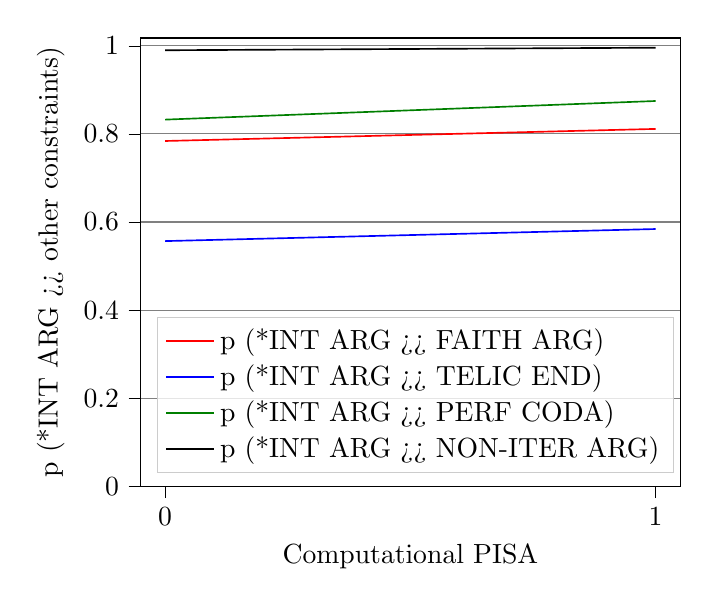
\begin{tikzpicture}

\definecolor{darkgray176}{RGB}{176,176,176}
\definecolor{gray}{RGB}{128,128,128}
\definecolor{green01270}{RGB}{0,127,0}
\definecolor{lightgray204}{RGB}{204,204,204}

\begin{axis}[
legend cell align={left},
legend style={
  fill opacity=0.8,
  draw opacity=1,
  text opacity=1,
  at={(0.03,0.03)},
  anchor=south west,
  draw=lightgray204
},
tick align=outside,
tick pos=left,
x grid style={darkgray176},
xlabel={Computational PISA},
xmin=-0.050000000065, xmax=1.050000001365,
xtick style={color=black},
xtick={1e-93,1.0000000013},
xticklabels={0,1},
y grid style={gray},
ylabel={p (*INT ARG >> other constraints)},
ymajorgrids,
ymin=0, ymax=1.01768426707614,
ytick style={color=black}
]
\addplot [semithick, red]
table {%
1e-93 0.783924357458075
1.0000000013 0.811345009309398
};
\addlegendentry{p (*INT ARG >> FAITH ARG)}
\addplot [semithick, blue]
table {%
1e-93 0.556704615448324
1.0000000013 0.584109403742447
};
\addlegendentry{p (*INT ARG >> TELIC END)}
\addplot [semithick, green01270]
table {%
1e-93 0.832454806686275
1.0000000013 0.874721634368817
};
\addlegendentry{p (*INT ARG >> PERF CODA)}
\addplot [semithick, black]
table {%
1e-93 0.98992820888467
1.0000000013 0.995732855093861
};
\addlegendentry{p (*INT ARG >> NON-ITER ARG)}
\end{axis}

\end{tikzpicture}
